\section{Results}

Table \ref{tab:res_prost} shows the obtained DSCs for the segmentation of the prostate
when the six trained models are used for the segmentation of the GE and Siemens dataset. 
The displayed DSC is computed from the validation subset when
the model is trained on the same dataset, and computed from the whole dataset when the
model is trained from a different dataset. 
\begin{table}[h]
    \centering
    \begin{tabular}{|l|c|c|}
         \hline
          & \multicolumn{2}{c|}{ \textbf{Tested on} } \\
         \hline
          \textbf{Trained with} &  GE & Siemens  \\
         \hline
         GE: wo/w DA & 0.748/0.758 & 0.305/0.34 \\
         \hline
         Siemens: wo/w DA & \textbf{0.150}/0.310 & 0.898/0.889\\
         \hline
         GE \& Siemens: wo/w DA & 0.753/0.739 & 0.904/\textbf{0.915}\\
         \hline
    \end{tabular}
    \caption{Dice Similarity Coefficients (DSC) between manual and CNN-generated 
    prostate contours for GE and Siemens MRI vendors datasets.}
    \label{tab:res_prost}
\end{table}
When the model is trained with examples from one dataset and used to segment
prostates from scans of the same MRI vendor the average DSCs are: 0.753 for GE 
and 0.893 for Siemens. When the datasets are combined during training, the 
average DSC are: .746 for GE and .909 for Siemens.
The results obtained for the Siemens dataset are comparable with 
current state of art methods for prostate segmentation. In the case the model is 
trained with examples from one dataset and used to segment scans from a diffent 
MRI vendor, then the average DSCs are low (0.322 and 0.169). This result exhibit 
how sensible the models
can be to subtle changes in the training dataset. It also displays the importance 
of testing how well the models generalize in other MRI vendors. 
The use of data augmentation improves the generalization of the models in most cases
but not with a clear tendency, further analysis is required. 

Table \ref{tab:res_pz} shows the obtained DSCs for the segmentation of the PZ
the six trained models.  The best DSCs (0.653 and 0.756) for segmenting the PZ of the prostate are obtained 
when the model is trained using the combined dataset.  

\begin{table}[h]
    \centering
    \begin{tabular}{|l|c|c|}
         \hline
          & \multicolumn{2}{c|}{ \textbf{Tested on} } \\
        \hline
         \textbf{Trained Width} &  GE & Siemens\\
         \hline
         GE: wo/w DA & 0.638/0.653& 0.331/\textbf{0.134} \\
         \hline
         Siemens: wo/w DA & 0.290/0.313 & 0.733/0.739\\
         \hline
         GE \& Siemens: wo/w DA & 0.648/0.654 & 0.743/\textbf{0.756}\\
         \hline
    \end{tabular}
    \caption{Dice Similarity Coefficients (DSC) between manual and CNN-generated 
    PZ contours for GE and Siemens}
    \label{tab:res_pz}
\end{table}

The average DSCs of all the PZ models are lower than the coefficients for 
segmenting the prostate, which implies that PZ segmentation is a more challenging task.

Figure \ref{fig:resseg} shows one example of a prosate segmentation on the
Siemens MRI vendor and a PZ segmentation on the GE MRI vendor. Both examples
are from the middle layer of the prostate, and their corresponding DSC are .903 and
.737.
\begin{figure}[h]
    \centering
    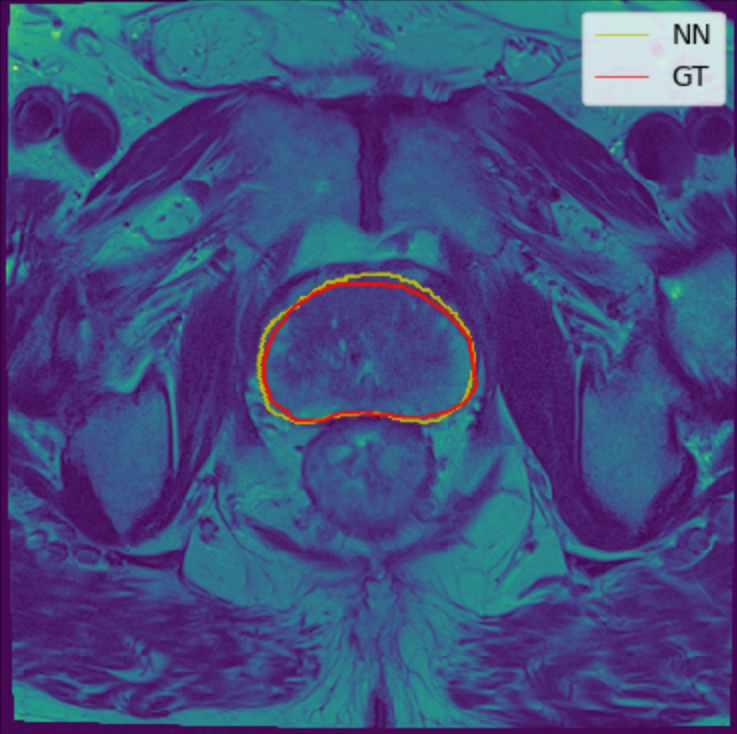
\includegraphics[totalheight=.18\textheight]{imgs/results/prosate.png}
    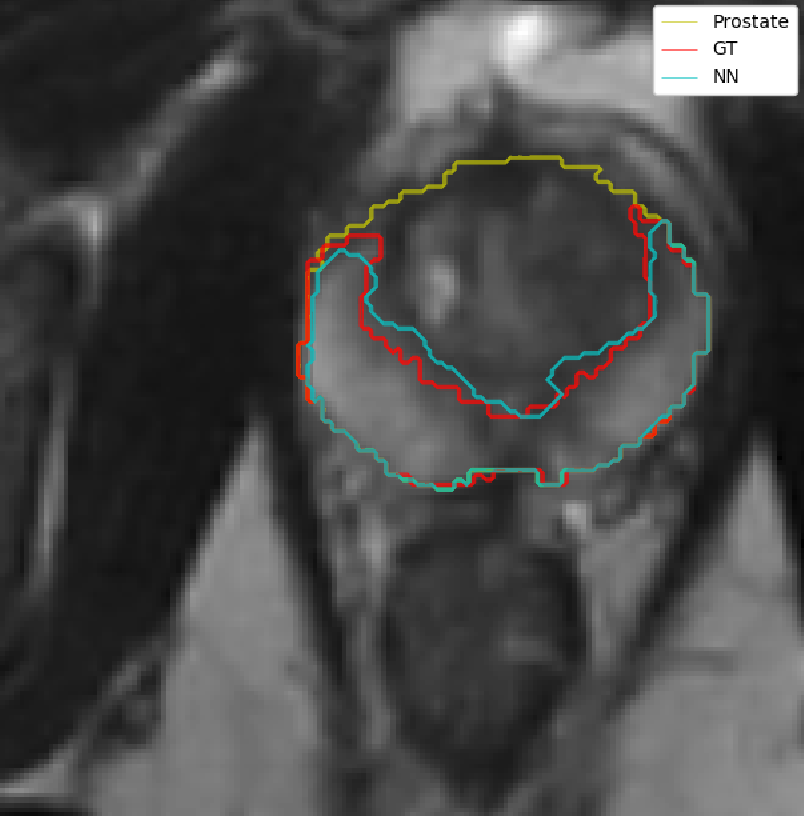
\includegraphics[totalheight=.18\textheight]{imgs/results/pz.png}
    \caption{Segmentation example of prosate (left) and pheripheral zone (right) on Siemens and GE
        MRI vendors respectively. The obtained DSCs for these examples are .903 for the prosate
        and .737 for the pheripheral zone.}
    \label{fig:resseg}
\end{figure}
